\section{Additional Confirmation Results}
\label{app:confirmation-details}

\subsection{Prediction, Repetition, and Student Cues}

Table~\ref{tab:absolute-losses} reports the absolute losses for all five
predictors on the three primary endpoints. Table~\ref{tab:primary-tests}
retains every prespecified primary comparison, including unresolved and negative
increments. All sources are equally weighted after averaging the matched
responses within each source. These tables use the original locked predictions
and full majority labels; the content-screened target is separate.

\begin{table}[htbp]\centering\small
\begin{tabular}{lrrr}\toprule
Predictor & Reveal & Elicit & Acknowledge \\
\midrule
Context & 0.153592 & 0.218731 & 0.182418 \\
Context + model default & 0.062317 & 0.089033 & 0.162597 \\
+ model $\times$ subject & 0.061894 & 0.092552 & 0.160458 \\
+ model $\times$ student state & 0.061463 & 0.092714 & 0.150724 \\
Context + training style & 0.138611 & 0.178259 & 0.178639 \\
\bottomrule\end{tabular}
\caption{Absolute source-averaged Brier losses on the 1,280 canonical
confirmation responses. Lower is better. The style competitor is descriptive.}
\label{tab:absolute-losses}\end{table}

\begin{table}[htbp]\centering\small
\begin{tabular}{llrrr}\toprule
Event & Increment & Brier gain & 95\% bootstrap interval & Holm $p$ \\
\midrule
Reveal & Default & 0.091275 & [0.071365, 0.109169] & $5.12\times10^{-10}$ \\
Reveal & Student state & 0.000431 & [-0.000373, 0.001299] & 0.325749 \\
Elicit & Default & 0.129698 & [0.121308, 0.137834] & $3.88\times10^{-24}$ \\
Elicit & Student state & -0.000163 & [-0.001007, 0.000726] & 0.640847 \\
Acknowledge & Default & 0.019821 & [0.014020, 0.025270] & $3.00\times10^{-7}$ \\
Acknowledge & Student state & 0.009734 & [0.005363, 0.013947] & 0.000192 \\
\bottomrule\end{tabular}
\caption{Six primary comparisons on 32 sources. Default adds model identity
to context; student state adds model-specific student-state responses to the
model-by-subject predictor. Tests are one-sided paired source tests with
Holm correction across six; bootstrap intervals are individual 95\% intervals.}
\label{tab:primary-tests}\end{table}

\begin{figure}[htbp]\centering
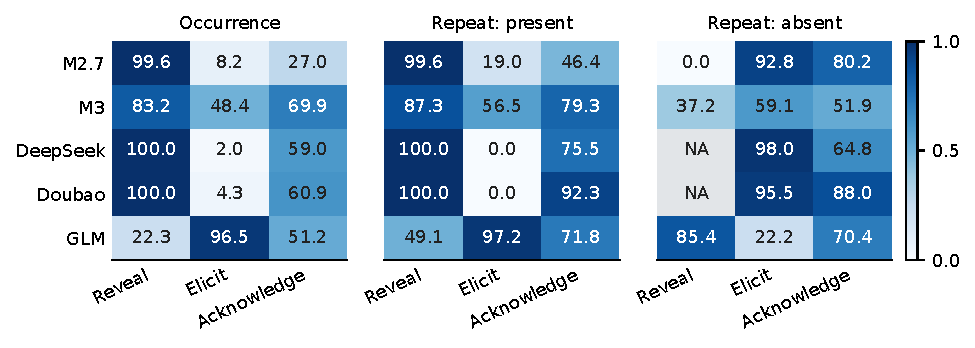
\includegraphics[width=\linewidth]{figures/confirmation_default_repetition_publication.pdf}
\caption{Canonical behavior rates and repeated-generation agreement (cells in
\%, color scale in probability units), with
256 answers and 128 input pairs per deployment on 32 sources. NA indicates
no denominator for agreement on absence, not zero agreement. Positive and
negative agreement prevent a large number of absent events from being
mistaken for recurrence of rare positive behavior. Source uncertainty is
retained in the accompanying numerical tables.}
\label{fig:default-repetition}\end{figure}

\begin{figure}[htbp]\centering
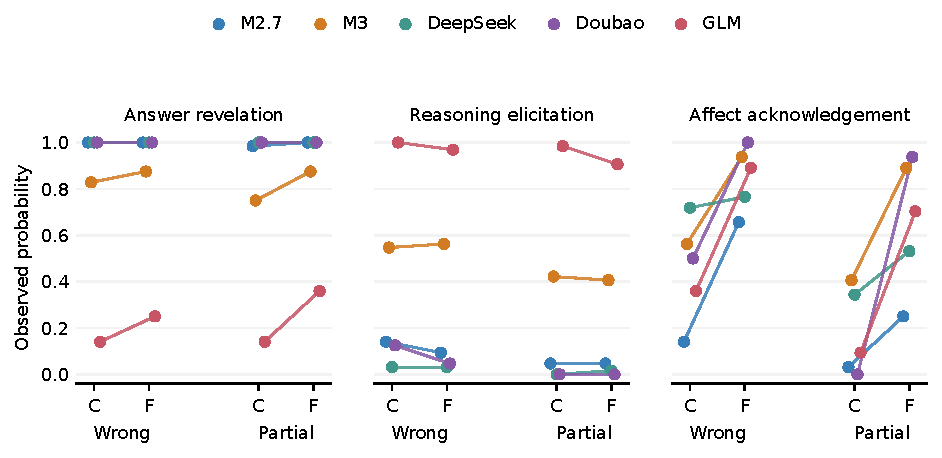
\includegraphics[width=\linewidth]{figures/confirmation_student_states_publication.pdf}
\caption{Canonical action rates for the four student-cue conditions. Each
point averages 64 responses over 32 sources. C denotes calm and F frustrated.
Lines connect calm and frustrated
inputs within a work state; work-state differences bundle correctness and
progress. These curves are descriptive and do not replace the locked
incremental prediction tests.}
\label{fig:student-states}\end{figure}

\subsection{Prompt Arms and Joint Actions}

Table~\ref{tab:matched-prompts} uses the same 16 source problems in every arm;
its canonical rates differ from the full 32-source profile. In EXPLAIN,
revelation is always present, so the elicitation rates equal the proportion
with both actions. In ASK, elicitation is always present, so the revelation
rates equal the proportion with both actions. Neither implication establishes
the order or pedagogical value of the actions.

\begin{table}[htbp]\centering\small
\begin{tabular}{llrrrrr}\toprule
Deployment & Event & Canonical & Neutral A & Neutral B & ASK & EXPLAIN \\
\midrule
M2.7 & Reveal & 100.0 & 98.4 & 97.7 & 7.0 & 100.0 \\
& Elicit & 9.4 & 10.9 & 15.6 & 100.0 & 5.5 \\
& Acknowledge & 25.0 & 33.6 & 27.3 & 10.2 & 18.0 \\
M3 & Reveal & 78.1 & 74.2 & 73.4 & 3.1 & 100.0 \\
& Elicit & 56.2 & 53.9 & 60.9 & 100.0 & 45.3 \\
& Acknowledge & 68.0 & 67.2 & 69.5 & 48.4 & 64.1 \\
DeepSeek & Reveal & 100.0 & 99.2 & 100.0 & 0.0 & 100.0 \\
& Elicit & 3.1 & 1.6 & 3.9 & 100.0 & 5.5 \\
& Acknowledge & 50.8 & 50.0 & 53.9 & 46.1 & 38.3 \\
Doubao & Reveal & 100.0 & 100.0 & 100.0 & 0.0 & 100.0 \\
& Elicit & 3.9 & 3.1 & 3.1 & 100.0 & 1.6 \\
& Acknowledge & 58.6 & 58.6 & 56.2 & 47.7 & 43.0 \\
GLM & Reveal & 27.3 & 28.9 & 43.0 & 0.0 & 100.0 \\
& Elicit & 95.3 & 97.7 & 91.4 & 100.0 & 62.5 \\
& Acknowledge & 49.2 & 56.2 & 64.8 & 47.7 & 46.1 \\
\bottomrule\end{tabular}
\caption{Matched prompt-arm event rates (\%). Every cell has 128 answers on
the same 16 sources. Abbreviations refer to the five specified deployments.}
\label{tab:matched-prompts}\end{table}

\begin{figure}[htbp]\centering
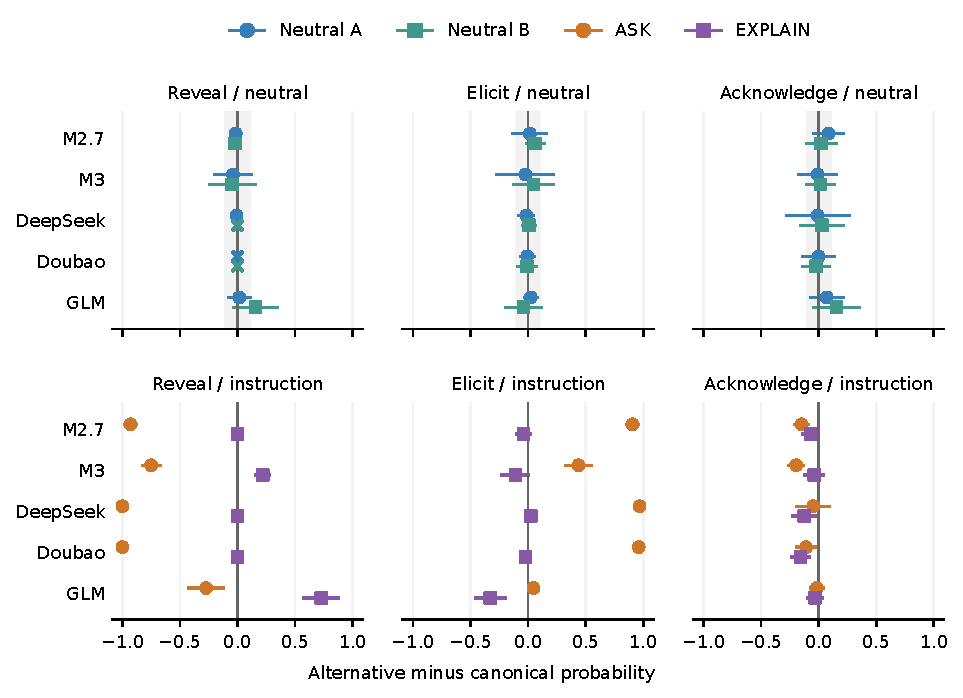
\includegraphics[width=\linewidth]{figures/confirmation_prompt_changes_publication.pdf}
\caption{Paired changes relative to canonical wording on the same 16 sources.
Neutral arms show nominal Bonferroni simultaneous 95\% paired-$t$ intervals
over 30 contrasts, with a $\pm0.10$ reference band. Explicit instruction arms
show descriptive 95\% paired-$t$ intervals. Crosses identify zero-variance
intervals; sparse-outcome undercoverage is not limited to those cases. These
intervals cannot establish population equivalence; the bounded-source check
below controls that interpretation.}
\label{fig:prompt-changes}\end{figure}

Three nominal neutral comparisons are degenerate. After excluding these,
seven comparisons still meet a nominal $t$-based tolerance criterion. None
meets the separate bounded-source rule: its simultaneous half-width is
0.9414 for the 30 contrasts. We therefore make no population-equivalence
claim for any neutral arm. The GLM neutral-B shifts are descriptive examples
of observed wording sensitivity, not proof of a population effect from a
selected unadjusted interval.

\subsection{Sensitivity to Coders, Deployments, and Training Sources}

The eight coding panels comprise three single coders, three leave-one-coder
panels, all-three soft labels, and exclusion of the generator's coder family.
Their default-gain ranges are reported in Section~\ref{sec:results}.
Conditional gain ranges are [0.000369, 0.000593] for revelation,
[-0.000301, 0.000002] for elicitation, and [0.006970, 0.010522] for
acknowledgement. Panel-specific forecasts were locked before confirmation;
labels and predictions are compared within their corresponding panel.

Across the five generator deletions, default-gain estimates span
[0.003942, 0.115447], [0.030800, 0.156526], and [0.001748, 0.028750] for
revelation, elicitation, and acknowledgement. These changes include refitting
the specified predictor on the reduced training-model panel before confirmation;
they are not predictions for unseen model identities. Conditional
acknowledgement gains span [0.002844, 0.012928]. The corresponding individual
source-bootstrap intervals exclude zero in all five deletions, but these
are supplemental intervals, not five additional primary hypothesis tests.
The default acknowledgement interval crosses zero without M2.7, and the
revelation default gain without GLM is small; the full-panel result is not
a claim of equal robustness across subsets.

The 200 training-source resamples yield 2.5--97.5 percentile ranges of
[0.086539, 0.092425], [0.126473, 0.131030], and [0.016673, 0.021398] for
the three default gains. Conditional ranges are [-0.001067, 0.000641],
[-0.002126, -0.000058], and [0.005422, 0.010389]. Sources are resampled
as groups with multiplicity weights; the original regularization ratio and
confirmation labels remain fixed. These ranges describe training-set
sensitivity and are not replacement confidence intervals for the six tests.

\subsection{Secondary Events, Expression Opportunities, and Sentinels}

\begin{table}[htbp]\centering\small
\begin{tabular}{lrrrrr}\toprule
Deployment & Explain & Choice & Qualify & Request & Ability claim \\
\midrule
M2.7 & 98.0 & 11.7 & 4.7 & 0.0 & 6.6 \\
M3 & 92.2 & 25.8 & 5.9 & 0.0 & 18.0 \\
DeepSeek & 96.9 & 4.3 & 9.4 & 0.0 & 2.0 \\
Doubao & 99.2 & 3.9 & 3.1 & 0.0 & 1.2 \\
GLM & 78.9 & 3.9 & 4.3 & 0.0 & 2.3 \\
\bottomrule\end{tabular}
\caption{All five secondary canonical event rates (\%), each based on
256 answers. Columns denote worked explanation, learner choice, epistemic
qualification, information request, and unsupported ability attribution.
Measurement quality varies by event; these are not validated personality axes.}
\label{tab:secondary-events}\end{table}

\begin{table}[htbp]\centering\small
\setlength{\tabcolsep}{4pt}
\begin{tabular}{llrrrrrr}\toprule
Subset & Sources/answers & D: R & D: E & D: A & S: R & S: E & S: A \\
\midrule
All canonical & 32/1280 & 0.09127 & 0.12970 & 0.01982 & 0.00043 & -0.00016 & 0.00973 \\
Mathematics & 8/320 & 0.11624 & 0.13892 & 0.01992 & 0.00062 & 0.00030 & 0.01380 \\
Exclude unanimous & 32/1255 & 0.09234 & 0.12948 & 0.02010 & 0.00047 & -0.00017 & 0.00987 \\
Exclude either & 32/1065 & 0.09535 & 0.13179 & 0.02068 & 0.00076 & 0.00023 & 0.00989 \\
Exclude either/uncertain & 32/1065 & 0.09535 & 0.13179 & 0.02068 & 0.00076 & 0.00023 & 0.00989 \\
\bottomrule\end{tabular}
\caption{All five content-sensitivity subsets, using unchanged locked
predictions. D denotes default versus context; S denotes student state versus
model-by-subject. R/E/A denote revelation, elicitation and acknowledgement.
Entries are source-equal Brier gains, not new hypothesis tests.}
\label{tab:content-subsets}\end{table}

Positive coder agreement on the full 4,040-response panel is 39.62--61.26\%
for epistemic qualification and 26.54--40.93\% for unsupported ability claims.
Their rates require particular caution. Information requests have
75.51--88.89\% positive agreement over the mixed full panel, which includes
the opportunity probes; this does not resolve the lack of natural pilot
positive examples or validate all missing-information detection.

No deployment requests missing information in the fully specified canonical
responses. On eight separate paired opportunity sources (16 responses per
deployment per condition), requests remain absent when the necessary facts
are supplied. When a necessary fact is withheld, request rates are 62.5\%
for M2.7, 93.8\% for M3, 25.0\% for DeepSeek, 12.5\% for Doubao, and
43.8\% for GLM. This bounded diagnostic shows why absence in the canonical
panel cannot establish an absence of information-seeking behavior. These
secondary rates are not population trait estimates.

Four training source problems are repeated as later sentinels, with two
requests per deployment at each stage. The paired-stage tables preserve
differences for every event and configuration. The sample is too small, and
the observations combine generation variation, coding variation, and possible
deployment drift, to attribute any change specifically to provider drift.
Moreover, the tutor generations preceded the later Gateway coding outage;
these sentinels cannot validate the stability of the coding deployments
across that outage.

\subsection{Mathematics and Content-Selection Sensitivity}
\label{app:content-results}



Table~\ref{tab:content-subsets} reports every selected subset.
Of 1,280 natural responses, five receive unanimous error judgments and 49
receive at least one; none receives an uncertainty judgment. The five
unanimous errors occupy five comparison slots. The 49 either-reviewer errors
occupy 43 slots, whose exclusion removes 215 answers because all five models
are removed together. All 32 sources retain observations. Per-model counts
(unanimous/either) are M2.7 2/17, M3 3/20, DeepSeek 0/0, Doubao 0/2, and
GLM 0/10, each out of 256 responses. These are reviewer flags, not an accuracy
ranking. Overall reviewer verdict agreement is 96.6\%, but error-positive
agreement is only $2(5)/(49+5)=18.5\%$, illustrating the effect of rare positives.
Each reviewer matches all six error and six no-error agent-authored controls;
these limited diagnostics do not resolve natural-response disagreement.

Across the three screens, the default-gain intervals remain above zero for
all three actions. Conditional acknowledgement intervals are [0.00551, 0.01405]
under unanimous-error exclusion and [0.00510, 0.01472] under either-error
exclusion. Conditional revelation and elicitation intervals span zero under
every screen. The last two screens are identical and are not independent
checks. Screening conditions on output judgments, changes the retained target,
and retains source-equal weighting; it does not remove ability as a cause.
The full primary tests are unchanged. The content-independent checkpoint's
all-canonical and mathematics tables agree with their completed counterparts
within $10^{-12}$, using the same routines rather than an independent implementation.
